% Options for packages loaded elsewhere
% Options for packages loaded elsewhere
\PassOptionsToPackage{unicode}{hyperref}
\PassOptionsToPackage{hyphens}{url}
\PassOptionsToPackage{dvipsnames,svgnames,x11names}{xcolor}
%
\documentclass[
  russian,
  letterpaper,
  DIV=11,
  numbers=noendperiod]{scrartcl}
\usepackage{xcolor}
\usepackage{amsmath,amssymb}
\setcounter{secnumdepth}{5}
\usepackage{iftex}
\ifPDFTeX
  \usepackage[T1]{fontenc}
  \usepackage[utf8]{inputenc}
  \usepackage{textcomp} % provide euro and other symbols
\else % if luatex or xetex
  \usepackage{unicode-math} % this also loads fontspec
  \defaultfontfeatures{Scale=MatchLowercase}
  \defaultfontfeatures[\rmfamily]{Ligatures=TeX,Scale=1}
\fi
\usepackage{lmodern}
\ifPDFTeX\else
  % xetex/luatex font selection
\fi
% Use upquote if available, for straight quotes in verbatim environments
\IfFileExists{upquote.sty}{\usepackage{upquote}}{}
\IfFileExists{microtype.sty}{% use microtype if available
  \usepackage[]{microtype}
  \UseMicrotypeSet[protrusion]{basicmath} % disable protrusion for tt fonts
}{}
\makeatletter
\@ifundefined{KOMAClassName}{% if non-KOMA class
  \IfFileExists{parskip.sty}{%
    \usepackage{parskip}
  }{% else
    \setlength{\parindent}{0pt}
    \setlength{\parskip}{6pt plus 2pt minus 1pt}}
}{% if KOMA class
  \KOMAoptions{parskip=half}}
\makeatother
% Make \paragraph and \subparagraph free-standing
\makeatletter
\ifx\paragraph\undefined\else
  \let\oldparagraph\paragraph
  \renewcommand{\paragraph}{
    \@ifstar
      \xxxParagraphStar
      \xxxParagraphNoStar
  }
  \newcommand{\xxxParagraphStar}[1]{\oldparagraph*{#1}\mbox{}}
  \newcommand{\xxxParagraphNoStar}[1]{\oldparagraph{#1}\mbox{}}
\fi
\ifx\subparagraph\undefined\else
  \let\oldsubparagraph\subparagraph
  \renewcommand{\subparagraph}{
    \@ifstar
      \xxxSubParagraphStar
      \xxxSubParagraphNoStar
  }
  \newcommand{\xxxSubParagraphStar}[1]{\oldsubparagraph*{#1}\mbox{}}
  \newcommand{\xxxSubParagraphNoStar}[1]{\oldsubparagraph{#1}\mbox{}}
\fi
\makeatother


\usepackage{longtable,booktabs,array}
\usepackage{calc} % for calculating minipage widths
% Correct order of tables after \paragraph or \subparagraph
\usepackage{etoolbox}
\makeatletter
\patchcmd\longtable{\par}{\if@noskipsec\mbox{}\fi\par}{}{}
\makeatother
% Allow footnotes in longtable head/foot
\IfFileExists{footnotehyper.sty}{\usepackage{footnotehyper}}{\usepackage{footnote}}
\makesavenoteenv{longtable}
\usepackage{graphicx}
\makeatletter
\newsavebox\pandoc@box
\newcommand*\pandocbounded[1]{% scales image to fit in text height/width
  \sbox\pandoc@box{#1}%
  \Gscale@div\@tempa{\textheight}{\dimexpr\ht\pandoc@box+\dp\pandoc@box\relax}%
  \Gscale@div\@tempb{\linewidth}{\wd\pandoc@box}%
  \ifdim\@tempb\p@<\@tempa\p@\let\@tempa\@tempb\fi% select the smaller of both
  \ifdim\@tempa\p@<\p@\scalebox{\@tempa}{\usebox\pandoc@box}%
  \else\usebox{\pandoc@box}%
  \fi%
}
% Set default figure placement to htbp
\def\fps@figure{htbp}
\makeatother



\ifLuaTeX
\usepackage[bidi=basic,provide=*]{babel}
\else
\usepackage[bidi=default,provide=*]{babel}
\fi
% get rid of language-specific shorthands (see #6817):
\let\LanguageShortHands\languageshorthands
\def\languageshorthands#1{}


\setlength{\emergencystretch}{3em} % prevent overfull lines

\providecommand{\tightlist}{%
  \setlength{\itemsep}{0pt}\setlength{\parskip}{0pt}}



 


\usepackage{fontspec}

\setsansfont{Palatino Linotype}[
    Path=../files/palatino/,
    Extension = .ttf,
    UprightFont=palatino-Roman,
    BoldFont=palatino-Bold,
    ItalicFont=palatino-Italic,
    BoldItalicFont=palatino-BoldItalic
]
\setmainfont{Palatino Linotype}[
    Path=../files/palatino/,
    Extension = .ttf,
    UprightFont=palatino-Roman,
    BoldFont=palatino-Bold,
    ItalicFont=palatino-Italic,
    BoldItalicFont=palatino-BoldItalic
]

\usepackage[textwidth=0.86\paperwidth, textheight=0.86\paperheight]{geometry}
\usepackage{fancyhdr}
\usepackage{hyperref}
\usepackage{fontawesome5}
\usepackage{graphicx}
\usepackage{amssymb}
\usepackage{amsmath}
\graphicspath{{../files/}}

\newcommand{\R}{\mathbb{R}}

% \pagenumbering{gobble}
\pagestyle{fancy}
\fancyhead{} % clear all header fields
\fancyhead[R]{\href{https://cu25.fmin.xyz}{\faGem[regular]} \hspace{0.04cm} \href{https://github.com/MerkulovDaniil/cu25}{\faGithub} \hspace{0.07cm} \href{https://t.me/fminxyz}{\faTelegram}}
\fancyhead[L]{\href{https://fmin.xyz}{
\includegraphics[height=0.35cm]{logo.pdf}} ~ 
\includegraphics[height=0.35cm]{logo_cu.pdf} \hspace{2pt} \textbf{Оптимизация для всех! ЦУ. 2025}}
\KOMAoption{captions}{tableheading}
\makeatletter
\@ifpackageloaded{tcolorbox}{}{\usepackage[skins,breakable]{tcolorbox}}
\@ifpackageloaded{fontawesome5}{}{\usepackage{fontawesome5}}
\definecolor{quarto-callout-color}{HTML}{909090}
\definecolor{quarto-callout-note-color}{HTML}{0758E5}
\definecolor{quarto-callout-important-color}{HTML}{CC1914}
\definecolor{quarto-callout-warning-color}{HTML}{EB9113}
\definecolor{quarto-callout-tip-color}{HTML}{00A047}
\definecolor{quarto-callout-caution-color}{HTML}{FC5300}
\definecolor{quarto-callout-color-frame}{HTML}{acacac}
\definecolor{quarto-callout-note-color-frame}{HTML}{4582ec}
\definecolor{quarto-callout-important-color-frame}{HTML}{d9534f}
\definecolor{quarto-callout-warning-color-frame}{HTML}{f0ad4e}
\definecolor{quarto-callout-tip-color-frame}{HTML}{02b875}
\definecolor{quarto-callout-caution-color-frame}{HTML}{fd7e14}
\makeatother
\makeatletter
\@ifpackageloaded{caption}{}{\usepackage{caption}}
\AtBeginDocument{%
\ifdefined\contentsname
  \renewcommand*\contentsname{Содержание}
\else
  \newcommand\contentsname{Содержание}
\fi
\ifdefined\listfigurename
  \renewcommand*\listfigurename{Список Иллюстраций}
\else
  \newcommand\listfigurename{Список Иллюстраций}
\fi
\ifdefined\listtablename
  \renewcommand*\listtablename{Список Таблиц}
\else
  \newcommand\listtablename{Список Таблиц}
\fi
\ifdefined\figurename
  \renewcommand*\figurename{Рисунок}
\else
  \newcommand\figurename{Рисунок}
\fi
\ifdefined\tablename
  \renewcommand*\tablename{Таблица}
\else
  \newcommand\tablename{Таблица}
\fi
}
\@ifpackageloaded{float}{}{\usepackage{float}}
\floatstyle{ruled}
\@ifundefined{c@chapter}{\newfloat{codelisting}{h}{lop}}{\newfloat{codelisting}{h}{lop}[chapter]}
\floatname{codelisting}{Список}
\newcommand*\listoflistings{\listof{codelisting}{Список Каталогов}}
\makeatother
\makeatletter
\makeatother
\makeatletter
\@ifpackageloaded{caption}{}{\usepackage{caption}}
\@ifpackageloaded{subcaption}{}{\usepackage{subcaption}}
\makeatother
\usepackage{bookmark}
\IfFileExists{xurl.sty}{\usepackage{xurl}}{} % add URL line breaks if available
\urlstyle{same}
\hypersetup{
  pdftitle={Условия оптимальности. Функция Лагранжа. Условия Каруша-Куна-Таккера},
  pdfauthor={Даня Меркулов},
  pdflang={ru},
  colorlinks=true,
  linkcolor={blue},
  filecolor={Maroon},
  citecolor={Blue},
  urlcolor={Blue},
  pdfcreator={LaTeX via pandoc}}


\title{Условия оптимальности. Функция Лагранжа. Условия
Каруша-Куна-Таккера}
\author{Даня Меркулов}
\date{}
\begin{document}
\maketitle


\begin{quote}
В этой работе совершенно отсутствуют какие бы то ни было чертежи.
Излагаемые мною методы не требуют ни построений, ни геометрических или
механических рассуждений; они требуют только алгебраических операций,
подчиненных планомерному и однообразному алгоритму.
\end{quote}

---\emph{Предисловие к ``Аналитической механике''}

\begin{figure}[H]

{\centering 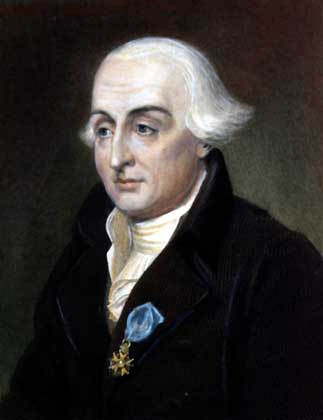
\includegraphics[width=0.5\linewidth,height=\textheight,keepaspectratio]{lagrange.jpg}

}

\caption{Жозеф Луи Лагранж}

\end{figure}%

\section{Условия
оптимальности}\label{ux443ux441ux43bux43eux432ux438ux44f-ux43eux43fux442ux438ux43cux430ux43bux44cux43dux43eux441ux442ux438}

\subsection{Теория}\label{ux442ux435ux43eux440ux438ux44f}

\begin{figure}[H]

{\centering \pandocbounded{\includegraphics[keepaspectratio]{"Local minima_ru.pdf"}}

}

\caption{Иллюстрация различных стационарных (критических) точек}

\end{figure}%

\[
f(x) \to \min\limits_{x \in S}
\]

Множество \(S\) обычно называется \textbf{допустимым множеством} (или
\textbf{бюджетным множеством}).

Мы говорим, что задача имеет решение, если бюджетное множество, в
котором достигается минимум или инфимум данной функции, \textbf{не
пусто}: \(x^* \in S\).

\begin{itemize}
\tightlist
\item
  Точка \(x^*\) является \textbf{глобальным минимумом}, если
  \(f(x^*) \leq f(x)\) для всех \(x \in S\).
\item
  Точка \(x^*\) является \textbf{локальным минимумом}, если существует
  окрестность \(N\) точки \(x^*\) такая, что \(f(x^*) \leq f(x)\) для
  всех \(x \in N \cap S\).
\item
  Точка \(x^*\) является \textbf{строгим локальным минимумом}, если
  существует окрестность \(N\) точки \(x^*\) такая, что
  \(f(x^*) < f(x)\) для всех \(x \in N \cap S\) с \(x \neq x^*\).
\item
  Мы называем точку \(x^*\) \textbf{стационарной точкой} (или
  критической точкой), если \(\nabla f(x^*) = 0\). Любой локальный
  минимум дифференцируемой функции должен быть стационарной точкой.
\end{itemize}

\subsection{Теорема Вейерштрасса об экстремальных
значениях}\label{ux442ux435ux43eux440ux435ux43cux430-ux432ux435ux439ux435ux440ux448ux442ux440ux430ux441ux441ux430-ux43eux431-ux44dux43aux441ux442ux440ux435ux43cux430ux43bux44cux43dux44bux445-ux437ux43dux430ux447ux435ux43dux438ux44fux445}

\begin{tcolorbox}[enhanced jigsaw, opacityback=0, coltitle=black, left=2mm, colframe=quarto-callout-color-frame, rightrule=.15mm, titlerule=0mm, leftrule=.75mm, breakable, colback=white, bottomrule=.15mm, bottomtitle=1mm, toptitle=1mm, opacitybacktitle=0.6, title=\textcolor{quarto-callout-color}{\faInfo}\hspace{0.5em}{Theorem}, colbacktitle=quarto-callout-color!10!white, arc=.35mm, toprule=.15mm]

Пусть \(S \subset \mathbb{R}^n\) - компактное множество и \(f(x)\) -
непрерывная функция на \(S\). Тогда точка глобального минимума функции
\(f(x)\) на \(S\) существует.

\end{tcolorbox}

\begin{figure}[H]

{\centering \pandocbounded{
\includegraphics[keepaspectratio]{goodnews.png}}

}

\caption{Многие практические задачи теоретически разрешимы}

\end{figure}%

\begin{tcolorbox}[enhanced jigsaw, opacityback=0, coltitle=black, left=2mm, colframe=quarto-callout-color-frame, rightrule=.15mm, titlerule=0mm, leftrule=.75mm, breakable, colback=white, bottomrule=.15mm, bottomtitle=1mm, toptitle=1mm, opacitybacktitle=0.6, title=\textcolor{quarto-callout-color}{\faInfo}\hspace{0.5em}{Теорема Тейлора}, colbacktitle=quarto-callout-color!10!white, arc=.35mm, toprule=.15mm]

Пусть \(f: \mathbb{R}^n \to \mathbb{R}\) - непрерывно дифференцируемая
функция и \(p \in \mathbb{R}^n\). Тогда мы имеем: \[
f(x + p) = f(x) + \nabla f(x + tp)^T p \quad \text{ для некоторого } t \in (0, 1)
\]

Кроме того, если \(f\) дважды непрерывно дифференцируема, то мы имеем:
\[
\nabla f(x + p) = \nabla f(x) + \int_0^1 \nabla^2 f(x + tp)p \, dt
\]

\[
f(x + p) = f(x) + \nabla f(x)^T p + \frac{1}{2} p^T \nabla^2 f(x + tp) p
\]

для некоторого \(t \in (0, 1)\).

\end{tcolorbox}

\section{Безусловная
оптимизация}\label{ux431ux435ux437ux443ux441ux43bux43eux432ux43dux430ux44f-ux43eux43fux442ux438ux43cux438ux437ux430ux446ux438ux44f}

\subsection{Необходимые
условия}\label{ux43dux435ux43eux431ux445ux43eux434ux438ux43cux44bux435-ux443ux441ux43bux43eux432ux438ux44f}

\begin{tcolorbox}[enhanced jigsaw, opacityback=0, coltitle=black, left=2mm, colframe=quarto-callout-color-frame, rightrule=.15mm, titlerule=0mm, leftrule=.75mm, breakable, colback=white, bottomrule=.15mm, bottomtitle=1mm, toptitle=1mm, opacitybacktitle=0.6, title=\textcolor{quarto-callout-color}{\faInfo}\hspace{0.5em}{Необходимое условие оптимальности первого порядка}, colbacktitle=quarto-callout-color!10!white, arc=.35mm, toprule=.15mm]

Если \(x^*\) - локальный минимум и \(f\) непрерывно дифференцируема в
открытой окрестности, то \[
\nabla f(x^*) = 0
\]

\textbf{Доказательство}

Предположим от противного, что \(\nabla f(x^*) \neq 0\). Определим
вектор \(p = -\nabla f(x^*)\) и заметим, что \[
p^T \nabla f(x^*) = -\| \nabla f(x^*) \|^2 < 0
\]

Поскольку \(\nabla f\) непрерывна в окрестности \(x^*\), существует
скаляр \(T > 0\) такой, что \[
p^T \nabla f(x^* + tp) < 0, \text{ для всех }\; t \in [0,T]
\]

Для любого \(\bar{t} \in (0, T]\), мы имеем по теореме Тейлора, что \[
f(x^* + \bar{t}p) = f(x^*) + \bar{t}\, p^T \, \nabla f(x^* + tp), \text{ для некоторого }\; t \in (0,\bar{t})
\]

Следовательно, \(f(x^* + \bar{t}p) < f(x^*)\) для всех
\(\bar{t} \in (0, T]\). Мы нашли направление из \(x^*\) вдоль которого
\(f\) убывает, поэтому \(x^*\) не является локальным минимумом, что
приводит к противоречию.

\end{tcolorbox}

\subsection{Достаточные
условия}\label{ux434ux43eux441ux442ux430ux442ux43eux447ux43dux44bux435-ux443ux441ux43bux43eux432ux438ux44f}

\begin{tcolorbox}[enhanced jigsaw, opacityback=0, coltitle=black, left=2mm, colframe=quarto-callout-color-frame, rightrule=.15mm, titlerule=0mm, leftrule=.75mm, breakable, colback=white, bottomrule=.15mm, bottomtitle=1mm, toptitle=1mm, opacitybacktitle=0.6, title=\textcolor{quarto-callout-color}{\faInfo}\hspace{0.5em}{Достаточные условия оптимальности второго порядка}, colbacktitle=quarto-callout-color!10!white, arc=.35mm, toprule=.15mm]

Пусть \(\nabla^2 f\) непрерывна в открытой окрестности \(x^*\), и
выполнено \[
\nabla f(x^*) = 0 \quad \nabla^2 f(x^*) \succ 0.
\]

Тогда \(x^*\) является строгим локальным минимумом функции \(f\).

\textbf{Доказательство}

Поскольку гессиан непрерывен и положительно определен в \(x^*\), мы
можем выбрать радиус \(r > 0\) такой, что \(\nabla^2 f(x)\) остается
положительно определенным для всех \(x\) в открытом шаре
\(B = \{ z \mid \|z - x^*\| < r \}\). Возьмем любой ненулевой вектор
\(p\) с \(\|p\| < r\), тогда \(x^* + p \in B\) и поэтому

\[ 
f(x^* + p) = f(x^*) + p^T \nabla f(x^*) + \frac{1}{2} p^T \nabla^2 f(z) p
\]

\[ 
= f(x^*) + \frac{1}{2} p^T \nabla^2 f(z) p
\]

где \(z = x^* + tp\) для некоторого \(t \in (0,1)\). Поскольку
\(z \in B\), то \(p^T \nabla^2 f(z) p > 0\), и поэтому
\(f(x^* + p) > f(x^*)\), что доказывает утверждение.

\end{tcolorbox}

\subsection{Контрпример
Пеано}\label{ux43aux43eux43dux442ux440ux43fux440ux438ux43cux435ux440-ux43fux435ux430ux43dux43e}

Заметим, что если \(\nabla f(x^*) = 0\), \(\nabla^2 f(x^*) \succeq 0\)
(гессиан положительно полуопределён), то мы не можем быть уверены, что
\(x^*\) является локальным минимумом.

\[
f(x,y) = (2x^2 - y)(x^2 - y)
\]

Хотя поверхность не имеет локального минимума в начале координат, ее
пересечение с любой вертикальной плоскостью, проходящей через начало
координат (плоскость с уравнением \(y=mx\) или \(x=0\)) является кривой,
которая имеет локальный минимум в начале координат. Другими словами,
если точка начинает движение в начале координат \((0,0)\) вдоль любой
прямой линии, то значение \((2x^2-y)(x^2 - y)\) будет увеличиваться в
начале движения. Тем не менее, \((0,0)\) не является локальным минимумом
функции, потому что движение вдоль параболы, такой как
\(y=\sqrt{2}x^2\), приведет к уменьшению значения функции.

\href{https://fmin.xyz/docs/theory/Optimality.html\#unconstrained-optimization}{\pandocbounded{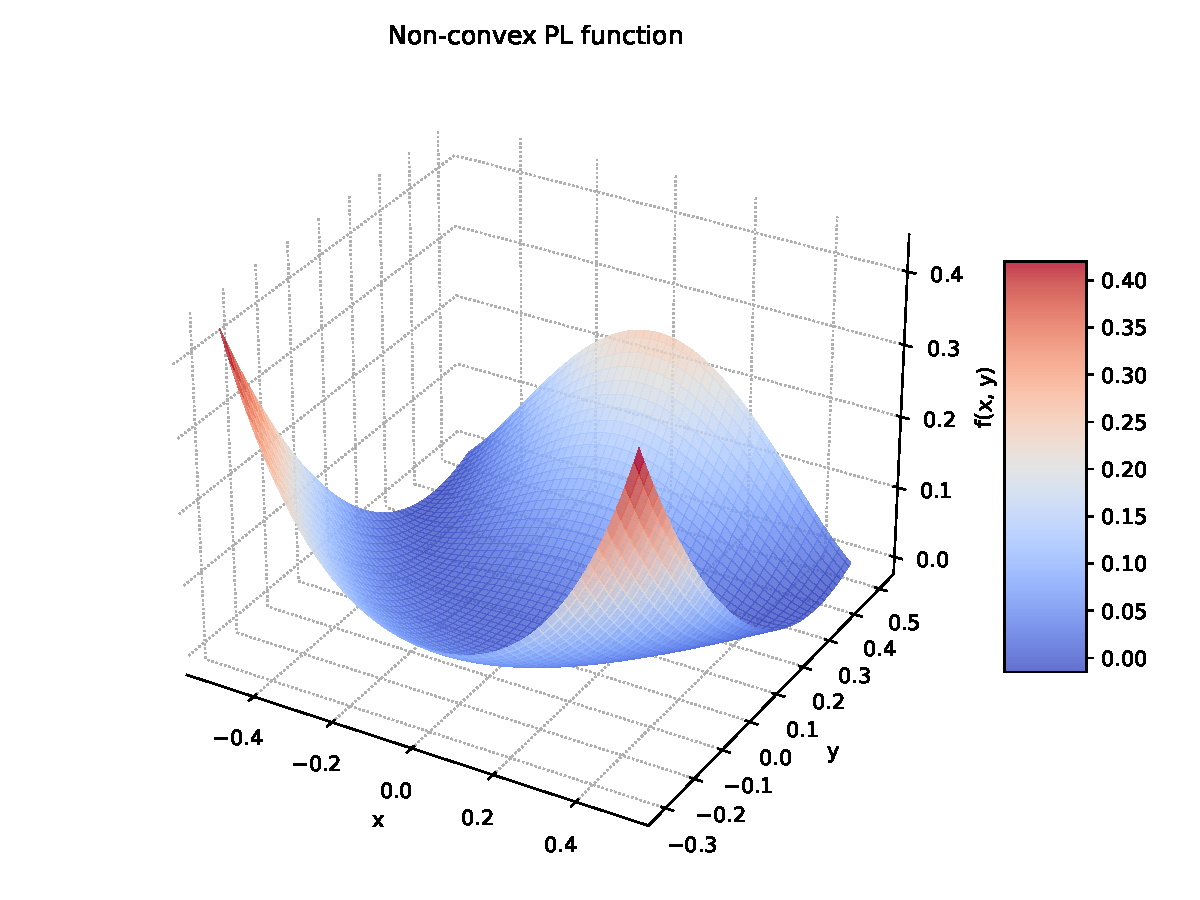
\includegraphics[keepaspectratio]{peano_surface.pdf}}}

\section{Условная
оптимизация}\label{ux443ux441ux43bux43eux432ux43dux430ux44f-ux43eux43fux442ux438ux43cux438ux437ux430ux446ux438ux44f}

\subsection{Общее условие локальной оптимальности первого
порядка}\label{ux43eux431ux449ux435ux435-ux443ux441ux43bux43eux432ux438ux435-ux43bux43eux43aux430ux43bux44cux43dux43eux439-ux43eux43fux442ux438ux43cux430ux43bux44cux43dux43eux441ux442ux438-ux43fux435ux440ux432ux43eux433ux43e-ux43fux43eux440ux44fux434ux43aux430}

Вектор \(d \in \mathbb{R}^n\) является допустимым направлением в точке
\(x^* \in S \subseteq \mathbb{R}^n\), если малые шаги вдоль \(d\) не
выводят нас за пределы \(S\).

Пусть \(S \subseteq \mathbb{R}^n\) и функция
\(f : \mathbb{R}^n \to \mathbb{R}\). Предположим, что \(x^* \in S\)
является точкой локального минимума для \(f\) над \(S\), и предположим
далее, что \(f\) непрерывно дифференцируема в окрестности \(x^*\).

\begin{enumerate}
\def\labelenumi{\arabic{enumi}.}
\tightlist
\item
  Тогда для любого допустимого направления \(d \in \mathbb{R}^n\) в
  \(x^*\) выполняется \(\nabla f(x^*)^\top d \geq 0\).
\item
  Если, кроме того, \(S\) выпукло, то\\
  \[
  \nabla f(x^*)^\top(x - x^*) \geq 0, \forall x \in S.
  \]
\end{enumerate}

\begin{figure}[H]

{\centering 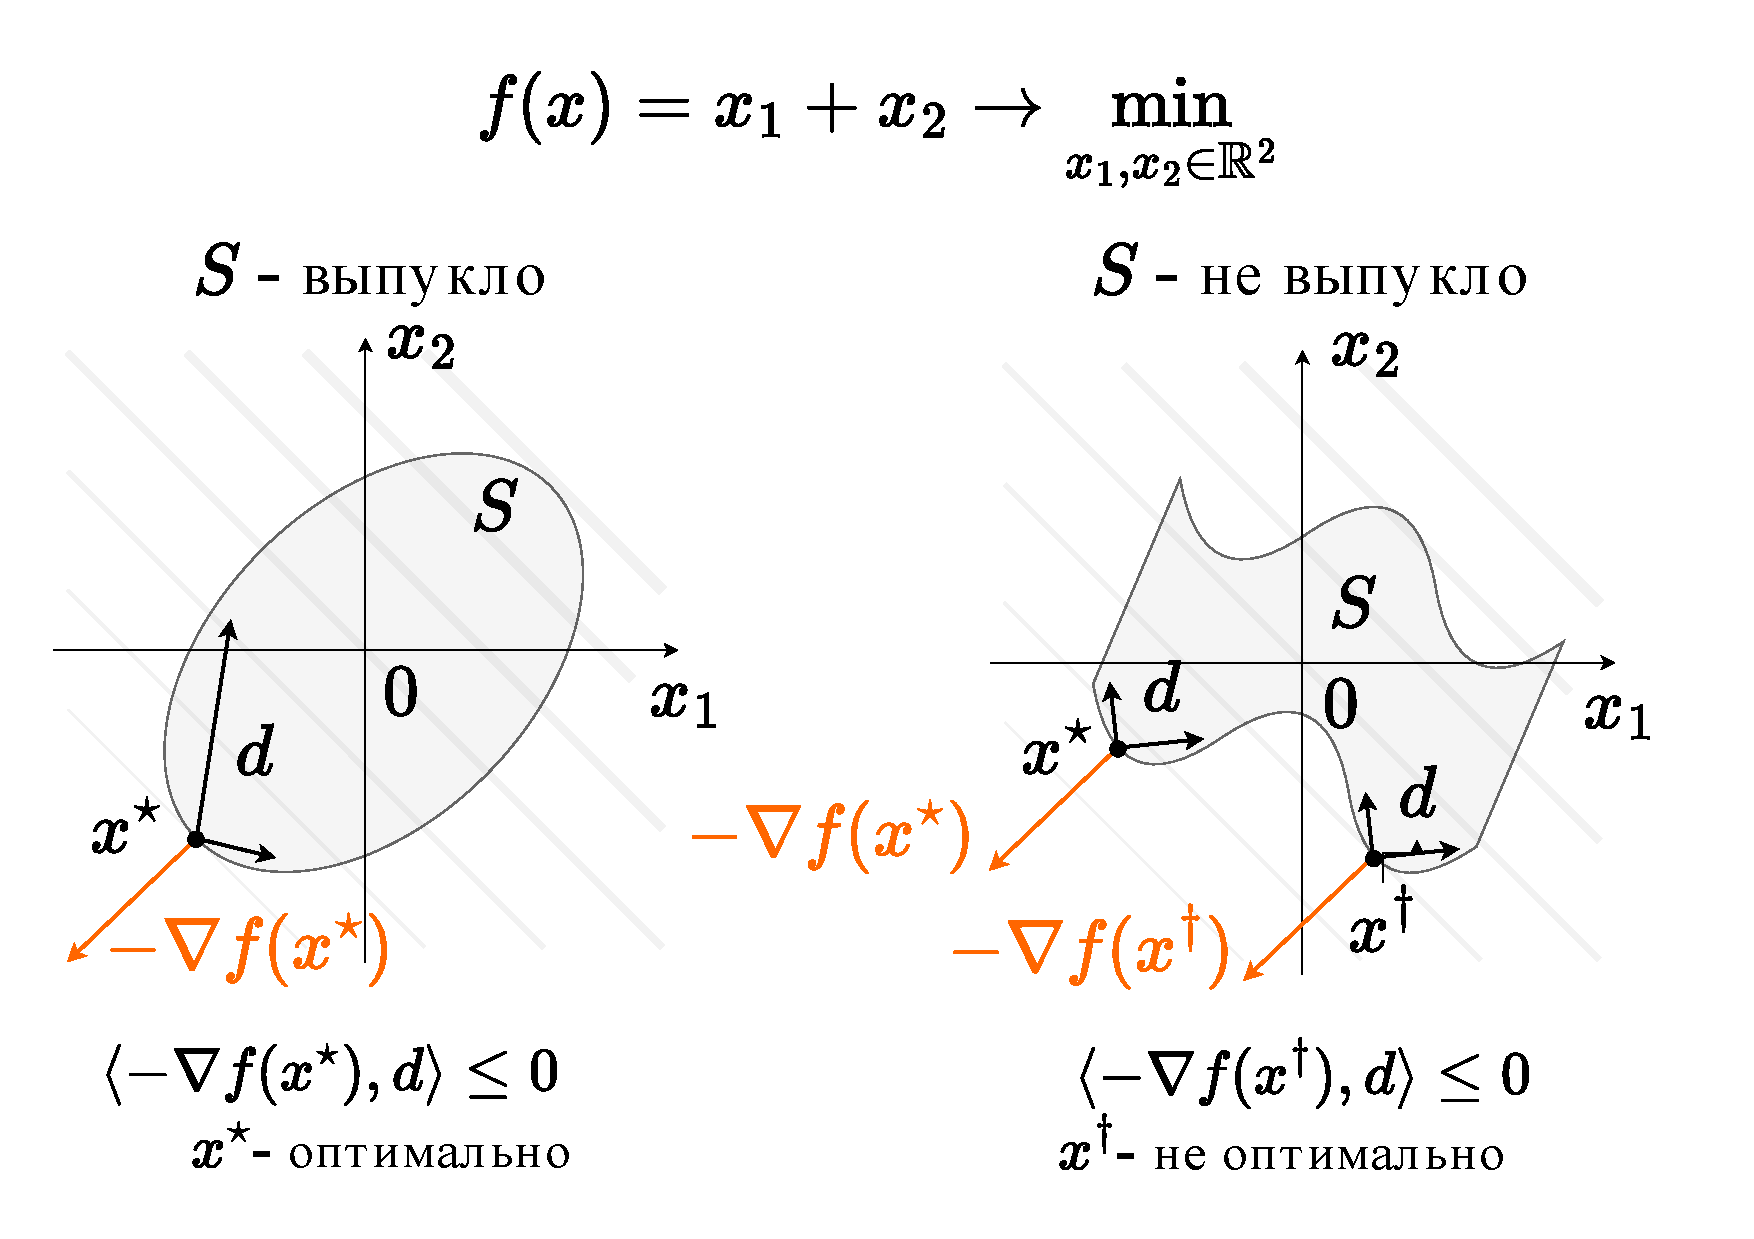
\includegraphics[width=0.7\linewidth,height=\textheight,keepaspectratio]{optimality_convexity_ru.pdf}

}

\caption{Общее условие локальной оптимальности первого порядка}

\end{figure}%

\subsection{Выпуклый
случай}\label{ux432ux44bux43fux443ux43aux43bux44bux439-ux441ux43bux443ux447ux430ux439}

Следует отметить, что в \textbf{выпуклом} случае (то есть при выпуклых
\(f\) и \(S\)) необходимое условие становится достаточным.

Еще один важный результат для выпуклого случая звучит следующим образом:
если \(f(x): S \to \mathbb{R}\) --- выпуклая функция, определённая на
выпуклом множестве \(S\), то:

\begin{itemize}
\tightlist
\item
  Любой локальный минимум является глобальным.
\item
  Множество локальных минимумов \(S^*\) выпукло.
\item
  Если \(f(x)\) --- строго или сильно выпуклая функция, то \(S^*\)
  содержит только одну точку: \(S^* = \{x^*\}\).
\end{itemize}

\subsection{Задачи с
ограничениями-равенствами}\label{ux437ux430ux434ux430ux447ux438-ux441-ux43eux433ux440ux430ux43dux438ux447ux435ux43dux438ux44fux43cux438-ux440ux430ux432ux435ux43dux441ux442ux432ux430ux43cux438}

В задачах без ограничений всё довольно интуитивно. В этом разделе мы
добавим одно ограничение-равенство, то есть:

\[
\begin{split}
& f(x) \to \min\limits_{x \in \mathbb{R}^n} \\
\text{s.t. } & h(x) = 0
\end{split}
\]

Мы попробуем проиллюстрировать подход к решению этой задачи через
простой пример с \(f(x) = x_1 + x_2\) и \(h(x) = x_1^2 + x_2^2 - 2\).

\begin{figure}[H]

{\centering \pandocbounded{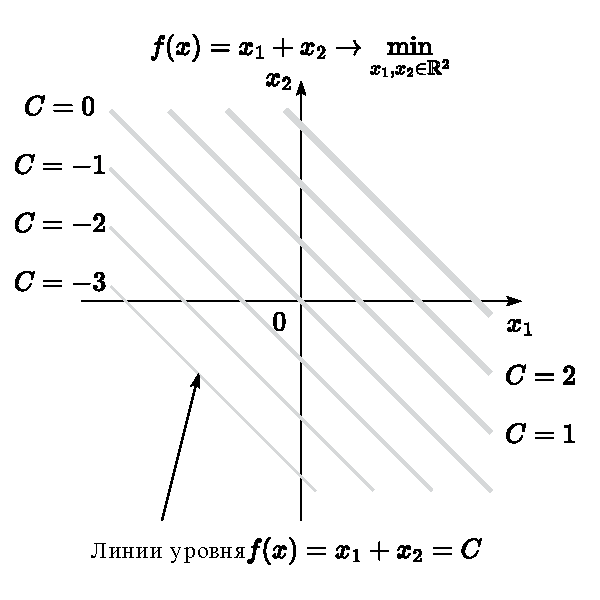
\includegraphics[keepaspectratio]{eq_constraint_1_ru.pdf}}

}

\caption{Иллюстрация ККТ}

\end{figure}%

\begin{figure}[H]

{\centering 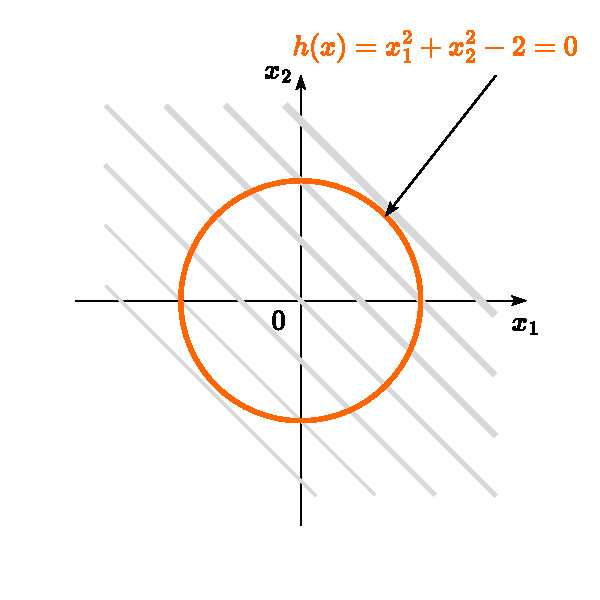
\includegraphics[width=0.5\linewidth,height=\textheight,keepaspectratio]{eq_constraint_2.pdf}

}

\caption{Иллюстрация ККТ}

\end{figure}%

\begin{figure}[H]

{\centering 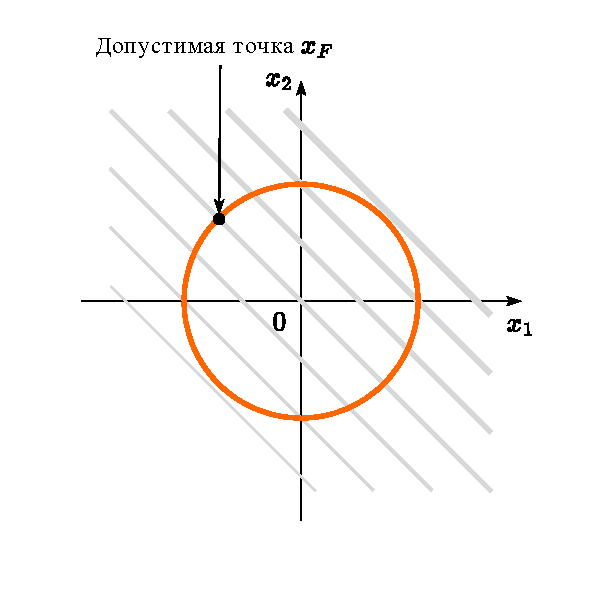
\includegraphics[width=0.5\linewidth,height=\textheight,keepaspectratio]{eq_constraint_3_ru.pdf}

}

\caption{Иллюстрация ККТ}

\end{figure}%

\begin{figure}[H]

{\centering 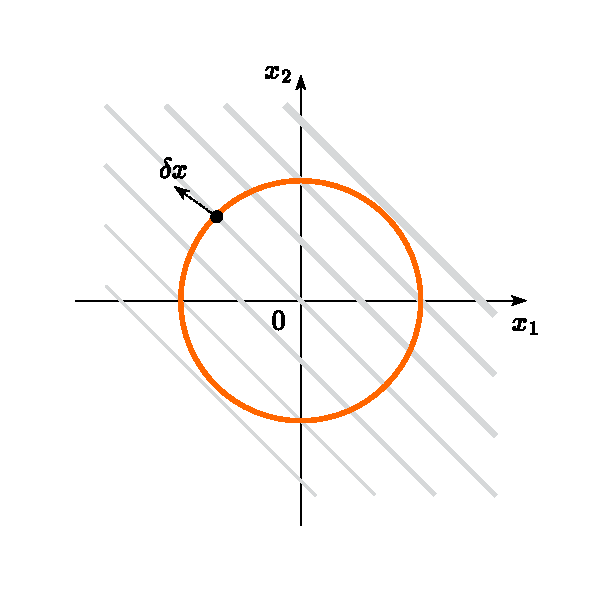
\includegraphics[width=0.5\linewidth,height=\textheight,keepaspectratio]{eq_constraint_4.pdf}

}

\caption{Иллюстрация ККТ}

\end{figure}%

\begin{figure}[H]

{\centering 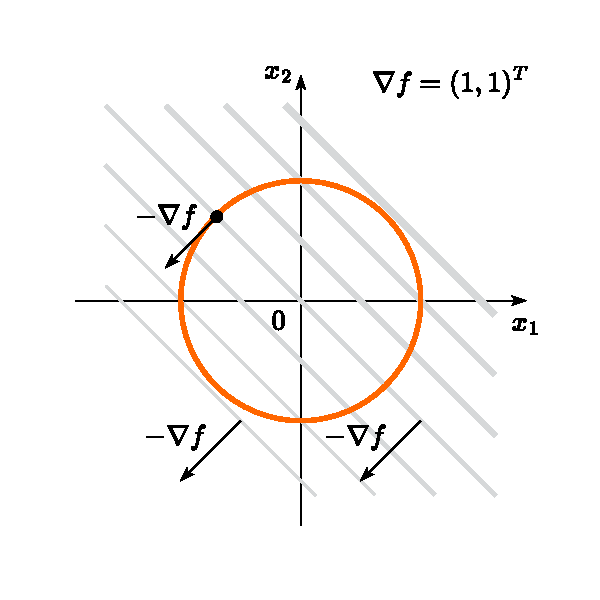
\includegraphics[width=0.5\linewidth,height=\textheight,keepaspectratio]{eq_constraint_5.pdf}

}

\caption{Иллюстрация ККТ}

\end{figure}%

\begin{figure}[H]

{\centering 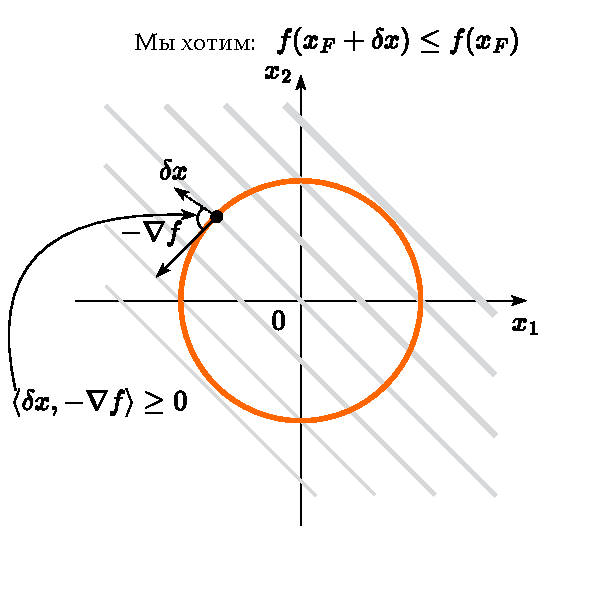
\includegraphics[width=0.5\linewidth,height=\textheight,keepaspectratio]{eq_constraint_6_ru.pdf}

}

\caption{Иллюстрация ККТ}

\end{figure}%

\begin{figure}[H]

{\centering 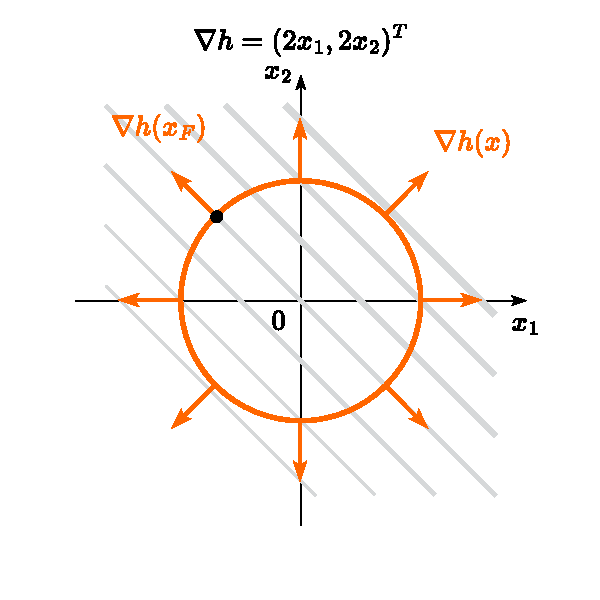
\includegraphics[width=0.5\linewidth,height=\textheight,keepaspectratio]{eq_constraint_7.pdf}

}

\caption{Иллюстрация ККТ}

\end{figure}%

\begin{figure}[H]

{\centering 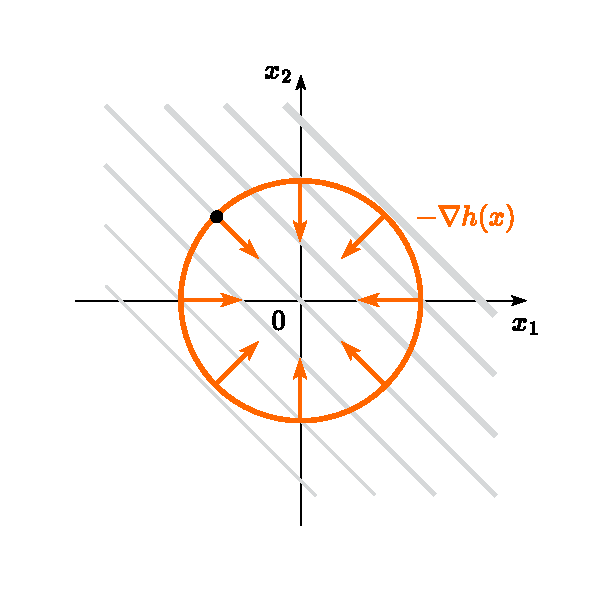
\includegraphics[width=0.5\linewidth,height=\textheight,keepaspectratio]{eq_constraint_8.pdf}

}

\caption{Иллюстрация ККТ}

\end{figure}%

\begin{figure}[H]

{\centering 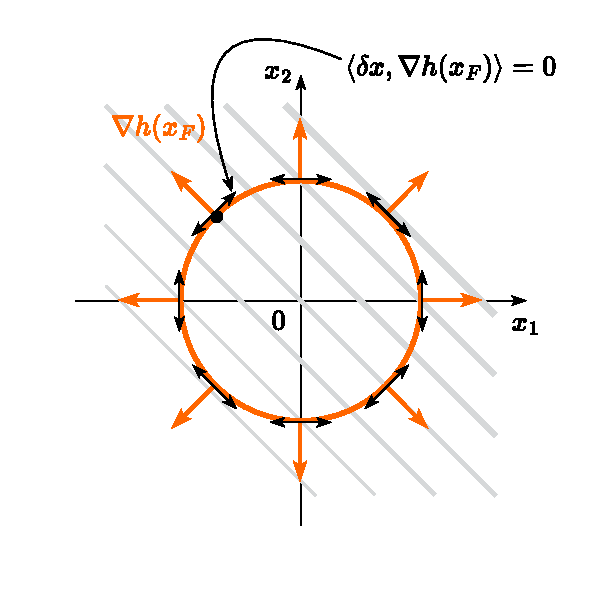
\includegraphics[width=0.5\linewidth,height=\textheight,keepaspectratio]{eq_constraint_9.pdf}

}

\caption{Иллюстрация ККТ}

\end{figure}%

В общем случае, чтобы двигаться от \(x_F\) вдоль допустимого множества и
уменьшать значение функции, необходимо обеспечить два условия:

\[
\langle \delta x, \nabla h(x_F) \rangle = 0
\]

\[
\langle \delta x, - \nabla f(x_F) \rangle > 0
\]

Предположим, что в процессе такого движения мы пришли в точку, где

\[
-\nabla f(x) = \nu \nabla h(x)
\]

\[
\langle  \delta x, - \nabla f(x)\rangle = \langle  \delta x, \nu\nabla h(x)\rangle = 0  
\]

Тогда мы достигли такой точки допустимого множества, из которой нельзя
уменьшить значение функции при допустимых малых сдвигах. Это и есть
условие локального минимума в задаче с ограничением.

\begin{figure}[H]

{\centering \pandocbounded{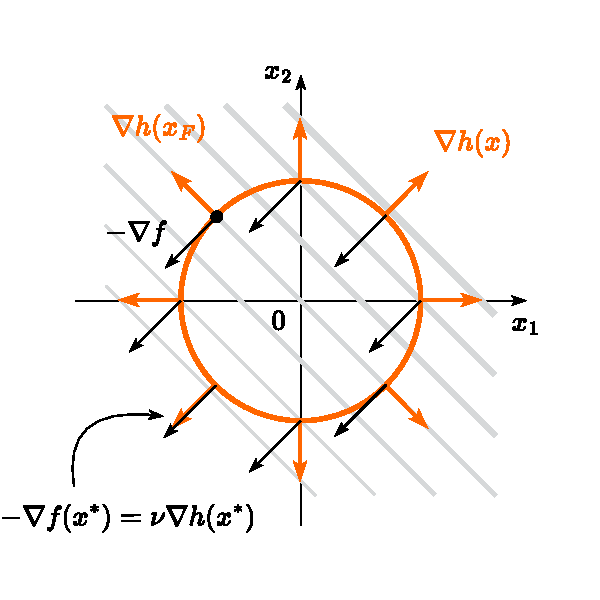
\includegraphics[keepaspectratio]{eq_constraint_10.pdf}}

}

\caption{Иллюстрация ККТ}

\end{figure}%

\subsection{Лагранжиан}\label{ux43bux430ux433ux440ux430ux43dux436ux438ux430ux43d}

Давайте определим лагранжиан (для удобства): \[
L(x, \nu) = f(x) + \nu h(x)
\]

Если задача \emph{регулярная} (мы определим это понятие позже) и точка
\(x^*\) является локальным минимумом для описанной выше задачи, то
существует \(\nu^*\):

\[
\begin{split}
 \text{Необходимые условия} \\
 \nabla_x L(x^*, \nu^*) = 0 \text{ это мы уже написали выше}\\
 \nabla_\nu L(x^*, \nu^*) = 0 \text{ бюджетное ограничение} \\
% \uncover<+->{& \text{Достаточные условия}}\\
% \uncover<+->{& \langle y , \nabla^2_{xx} L(x^*, \nu^*) y \rangle > 0,}\\
% \uncover<+->{& \forall y \neq 0 \in \mathbb{R}^n : \nabla h(x^*)^\top y = 0}
\end{split}
\] Важно отметить, что \(L(x^*, \nu^*) = f(x^*)\).

\[
\tag{ECP}
\begin{split}
& f(x) \to \min\limits_{x \in \mathbb{R}^n} \\
\text{s.t. } & h_i(x) = 0, \; i = 1,\ldots, p
\end{split}
\]

\[
L(x, \nu) = f(x) + \sum\limits_{i=1}^p\nu_i h_i(x) = f(x) + \nu^\top h(x)
\] Пусть \(f(x)\) и \(h_i(x)\) дважды дифференцируемы в точке \(x^*\) и
непрерывно дифференцируемы в некоторой окрестности \(x^*\). Условия
локального минимума для \(x \in \mathbb{R}^n, \nu \in \mathbb{R}^p\)
записываются как \[
\begin{split}
& \text{Необходимые условия} \\
& \nabla_x L(x^*, \nu^*) = 0 \\
& \nabla_\nu L(x^*, \nu^*) = 0
% & \text{Достаточные условия} \\
% & \langle y , \nabla^2_{xx} L(x^*, \nu^*) y \rangle > 0,\\
% & \forall y \neq 0 \in \mathbb{R}^n : \nabla h_i(x^*)^\top y = 0
\end{split}
\]

\subsection{Задача наименьших
квадратов}\label{ux437ux430ux434ux430ux447ux430-ux43dux430ux438ux43cux435ux43dux44cux448ux438ux445-ux43aux432ux430ux434ux440ux430ux442ux43eux432}

\begin{tcolorbox}[enhanced jigsaw, opacityback=0, coltitle=black, left=2mm, colframe=quarto-callout-color-frame, rightrule=.15mm, titlerule=0mm, leftrule=.75mm, breakable, colback=white, bottomrule=.15mm, bottomtitle=1mm, toptitle=1mm, opacitybacktitle=0.6, title=\textcolor{quarto-callout-color}{\faInfo}\hspace{0.5em}{Example}, colbacktitle=quarto-callout-color!10!white, arc=.35mm, toprule=.15mm]

Поставим задачу оптимизации и решим ее для линейной системы
\(Ax = b, A \in \mathbb{R}^{m \times n}\) для трех случаев (предполагая,
что матрица имеет полный ранг):

\begin{itemize}
\tightlist
\item
  \(m < n\)
\item
  \(m = n\)
\item
  \(m > n\)
\end{itemize}

\end{tcolorbox}

\section{Задачи с
ограничениями-неравенствами}\label{ux437ux430ux434ux430ux447ux438-ux441-ux43eux433ux440ux430ux43dux438ux447ux435ux43dux438ux44fux43cux438-ux43dux435ux440ux430ux432ux435ux43dux441ux442ux432ux430ux43cux438}

\subsection{Пример задачи с
ограничениями-неравенствами}\label{ux43fux440ux438ux43cux435ux440-ux437ux430ux434ux430ux447ux438-ux441-ux43eux433ux440ux430ux43dux438ux447ux435ux43dux438ux44fux43cux438-ux43dux435ux440ux430ux432ux435ux43dux441ux442ux432ux430ux43cux438}

\[
f(x) = x_1^2 + x_2^2 \;\;\;\; g(x) = x_1^2 + x_2^2 - 1
\]

\[
\begin{split}
& f(x) \to \min\limits_{x \in \mathbb{R}^n} \\
\text{s.t. } & g(x) \leq 0
\end{split}
\]

\subsection{Задачи с
ограничениями-неравенствами}\label{ux437ux430ux434ux430ux447ux438-ux441-ux43eux433ux440ux430ux43dux438ux447ux435ux43dux438ux44fux43cux438-ux43dux435ux440ux430ux432ux435ux43dux441ux442ux432ux430ux43cux438-1}

\begin{figure}[H]

{\centering \pandocbounded{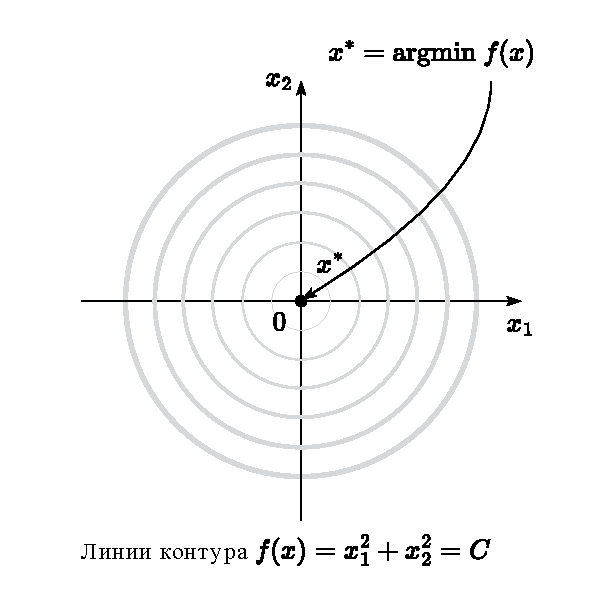
\includegraphics[keepaspectratio]{ineq_constr_1_ru.pdf}}

}

\caption{Иллюстрация ККТ (случай неравенства)}

\end{figure}%

\begin{figure}[H]

{\centering 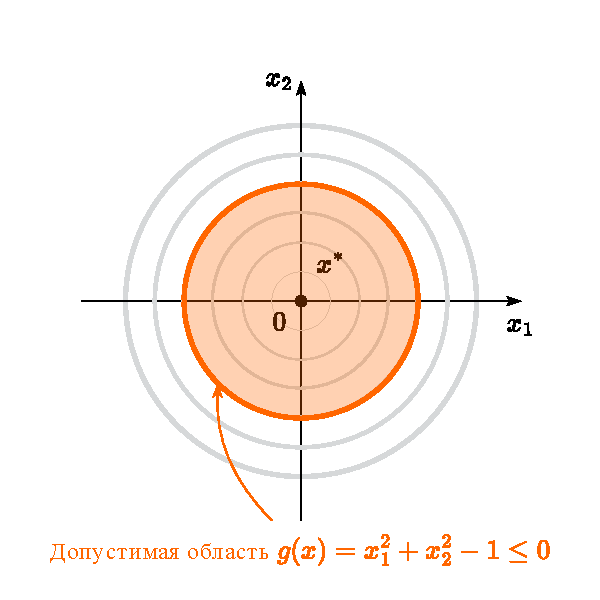
\includegraphics[width=0.5\linewidth,height=\textheight,keepaspectratio]{ineq_constr_2_ru.pdf}

}

\caption{Иллюстрация ККТ (случай неравенства)}

\end{figure}%

\begin{figure}[H]

{\centering 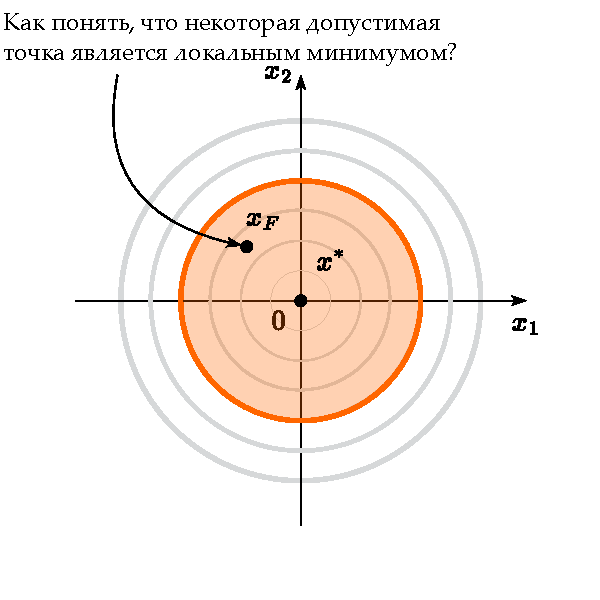
\includegraphics[width=0.5\linewidth,height=\textheight,keepaspectratio]{ineq_constr_3_ru.pdf}

}

\caption{Иллюстрация ККТ (случай неравенства)}

\end{figure}%

\begin{figure}[H]

{\centering 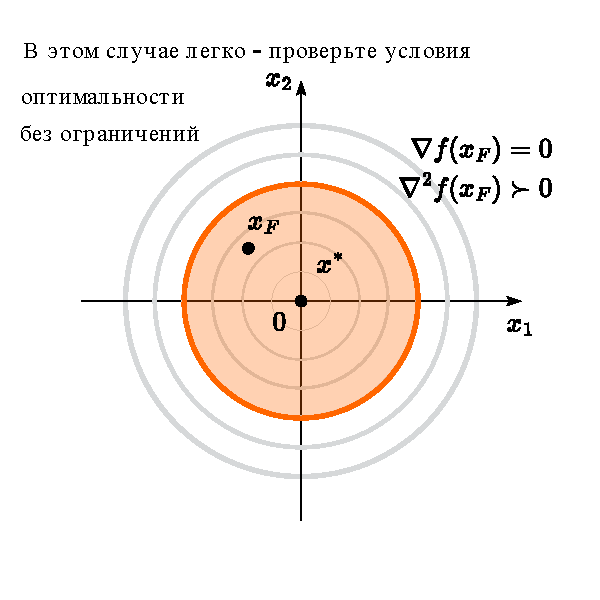
\includegraphics[width=0.5\linewidth,height=\textheight,keepaspectratio]{ineq_constr_4_ru.pdf}

}

\caption{Иллюстрация ККТ (случай неравенства)}

\end{figure}%

Таким образом, если ограничения типа неравенства неактивны в условной
задаче, то мы можем решать задачу без ограничений. Однако так бывает не
всегда. Рассмотрим второй простой пример. \[
f(x) = (x_1 - 1)^2 + (x_2 + 1)^2 \;\;\;\; g(x) = x_1^2 + x_2^2 - 1
\]

\[
\begin{split}
& f(x) \to \min\limits_{x \in \mathbb{R}^n} \\
\text{s.t. } & g(x) \leq 0
\end{split}
\]

\begin{figure}[H]

{\centering 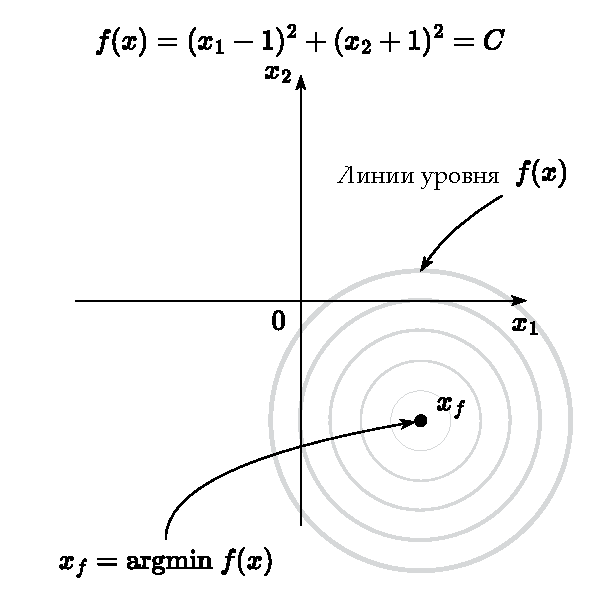
\includegraphics[width=0.5\linewidth,height=\textheight,keepaspectratio]{ineq_constr_5_ru.pdf}

}

\caption{Иллюстрация ККТ (случай неравенства)}

\end{figure}%

\begin{figure}[H]

{\centering 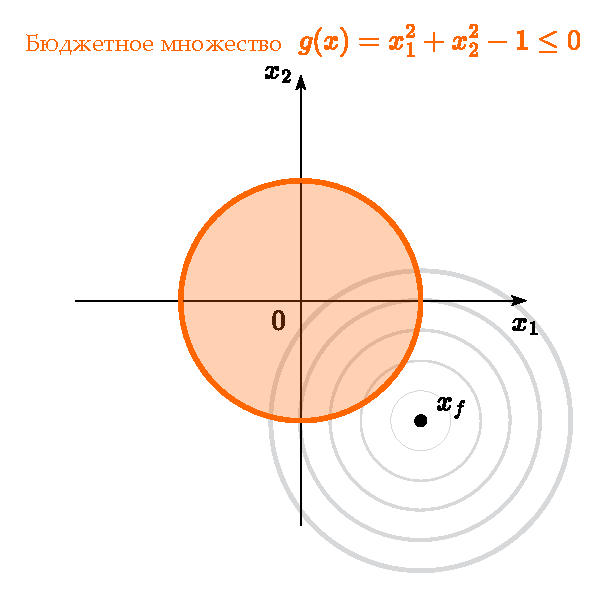
\includegraphics[width=0.5\linewidth,height=\textheight,keepaspectratio]{ineq_constr_6_ru.pdf}

}

\caption{Иллюстрация ККТ (случай неравенства)}

\end{figure}%

\begin{figure}[H]

{\centering 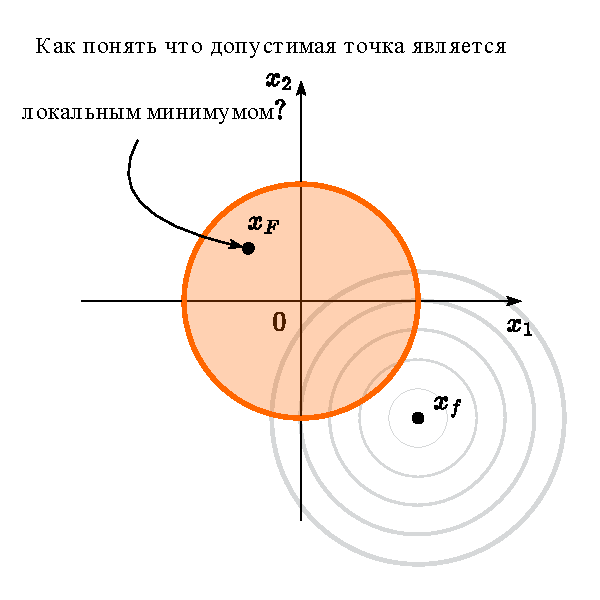
\includegraphics[width=0.5\linewidth,height=\textheight,keepaspectratio]{ineq_constr_7_ru.pdf}

}

\caption{Иллюстрация ККТ (случай неравенства)}

\end{figure}%

\begin{figure}[H]

{\centering 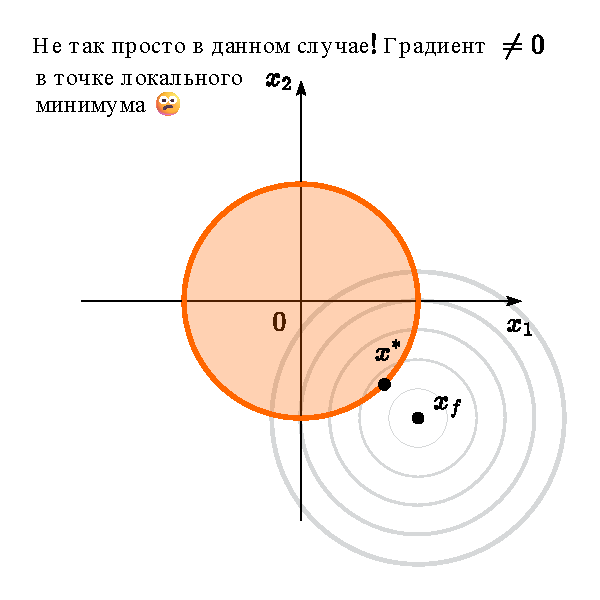
\includegraphics[width=0.5\linewidth,height=\textheight,keepaspectratio]{ineq_constr_8_ru.pdf}

}

\caption{Иллюстрация ККТ (случай неравенства)}

\end{figure}%

\begin{figure}[H]

{\centering 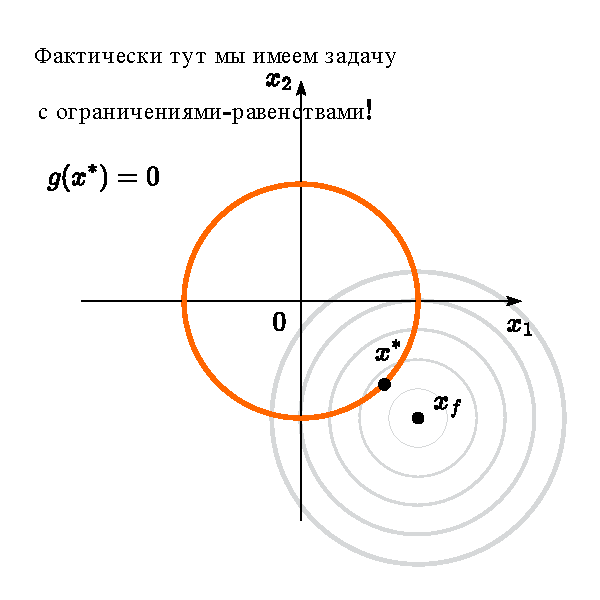
\includegraphics[width=0.5\linewidth,height=\textheight,keepaspectratio]{ineq_constr_9_ru.pdf}

}

\caption{Иллюстрация ККТ (случай неравенства)}

\end{figure}%

\begin{figure}[H]

{\centering 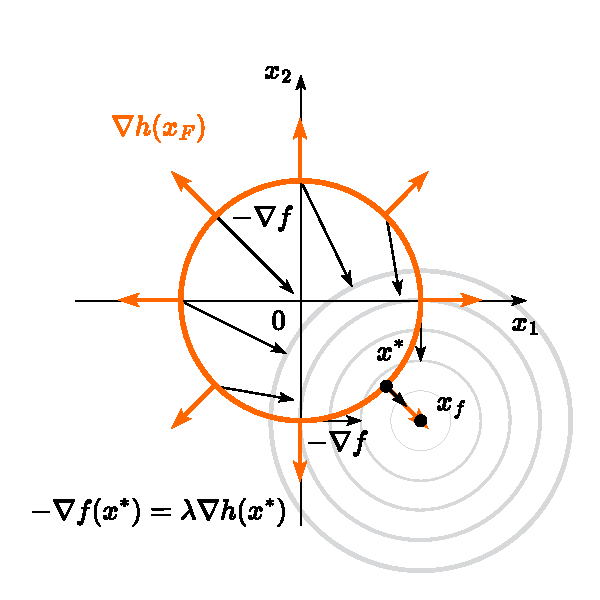
\includegraphics[width=0.5\linewidth,height=\textheight,keepaspectratio]{ineq_constr_10.pdf}

}

\caption{Иллюстрация ККТ (случай неравенства)}

\end{figure}%

\begin{figure}[H]

{\centering 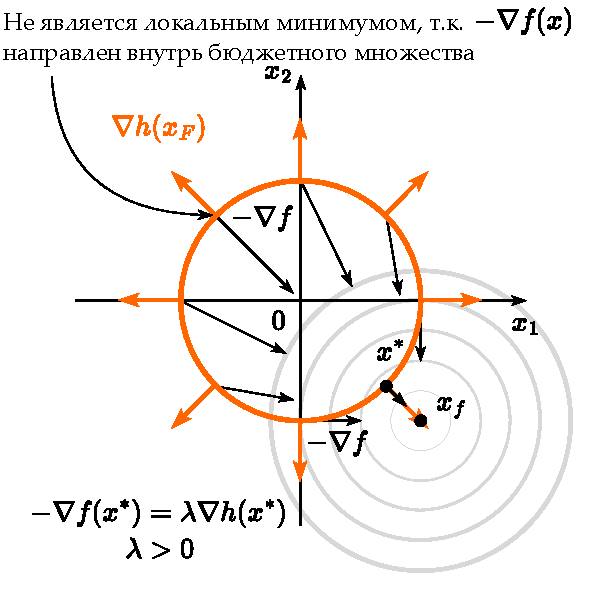
\includegraphics[width=0.5\linewidth,height=\textheight,keepaspectratio]{ineq_constr_11_ru.pdf}

}

\caption{Иллюстрация ККТ (случай неравенства)}

\end{figure}%

Итак, у нас есть задача: \[
\begin{split}
& f(x) \to \min\limits_{x \in \mathbb{R}^n} \\
\text{s.t. } & g(x) \leq 0
\end{split}
\] Два возможных случая:

\(g(x) \leq 0\) неактивно. \(g(x^*) < 0\)

\begin{itemize}
\tightlist
\item
  \(g(x^*) < 0\)
\item
  \(\nabla f(x^*) = 0\)
\item
  \(\nabla^2 f(x^*) > 0\)
\end{itemize}

\(g(x) \leq 0\) активно. \(g(x^*) = 0\)

\begin{itemize}
\tightlist
\item
  \(g(x^*) = 0\)
\item
  Необходимые условия: \(- \nabla f(x^*) = \lambda \nabla g(x^*)\),
  \(\lambda > 0\)
\end{itemize}

\subsection{Лагранжиан для задач с
ограничениями-неравенствами}\label{ux43bux430ux433ux440ux430ux43dux436ux438ux430ux43d-ux434ux43bux44f-ux437ux430ux434ux430ux447-ux441-ux43eux433ux440ux430ux43dux438ux447ux435ux43dux438ux44fux43cux438-ux43dux435ux440ux430ux432ux435ux43dux441ux442ux432ux430ux43cux438}

Объединяя два возможных случая, мы можем записать общие условия для
задачи: \[
\begin{split}
& f(x) \to \min\limits_{x \in \mathbb{R}^n} \\
\text{s.t. } & g(x) \leq 0
\end{split}
\] Определим функцию Лагранжа: \[
L(x, \lambda) = f(x) + \lambda g(x)
\] Классические условия Каруша-Куна-Таккера для локального минимума
\(x^*\), сформулированные при некоторых условиях регулярности, можно
записать следующим образом.

Если \(x^*\) является локальным минимумом для описанной выше задачи, то
существует единственный множитель Лагранжа \(\lambda^*\) такой, что: \[
\begin{split}
& (1) \; \nabla_x L (x^*, \lambda^*) = 0\\
& (2) \; \lambda^* \geq 0\\
& (3) \; \lambda^* g(x^*) = 0\\
& (4) \; g(x^*) \leq 0\\
% & (5) \; \forall y \in C(x^*):  \langle y , \nabla^2_{xx} L(x^*, \lambda^*) y \rangle > 0 \\
% &  \text{where } C(x^*) = \{y \ \in \mathbb{R}^n |  \nabla f(x^*)^\top y \leq 0 \text{ and } \forall i \in I(x^*):  \nabla g_i(x^*)^T y \leq 0 \} \text{ is the critical cone.} \\
% & I(x^*) = \{i \mid g_i(x^*) = 0\}
\end{split}
\]

\subsection{Общая
формулировка}\label{ux43eux431ux449ux430ux44f-ux444ux43eux440ux43cux443ux43bux438ux440ux43eux432ux43aux430}

\[
\begin{split}
& f_0(x) \to \min\limits_{x \in \mathbb{R}^n}\\
\text{s.t. } & f_i(x) \leq 0, \; i = 1,\ldots,m\\
& h_i(x) = 0, \; i = 1,\ldots, p
\end{split}
\] Данная формулировка является общей задачей математического
программирования.

Решение включает в себя построение лагранжиана: \[
L(x, \lambda, \nu) = f_0(x) + \sum\limits_{i=1}^m \lambda_i f_i(x) + \sum\limits_{i=1}^p\nu_i h_i(x)
\]

\subsection{Необходимые
условия}\label{ux43dux435ux43eux431ux445ux43eux434ux438ux43cux44bux435-ux443ux441ux43bux43eux432ux438ux44f-1}

Пусть \(x^*\), \((\lambda^*, \nu^*)\) является решением задачи
математического программирования с нулевым зазором двойственности
(оптимальное значение для исходной задачи \(p^*\) равно оптимальному
значению для двойственной задачи \(d^*\)). Пусть также функции
\(f_0, f_i, h_i\) дифференцируемы.

\begin{itemize}
\tightlist
\item
  \(\nabla_x L(x^*, \lambda^*, \nu^*) = 0\)
\item
  \(\nabla_\nu L(x^*, \lambda^*, \nu^*) = 0\)
\item
  \(\lambda^*_i \geq 0, i = 1,\ldots,m\)
\item
  \(\lambda^*_i f_i(x^*) = 0, i = 1,\ldots,m\)
\item
  \(f_i(x^*) \leq 0, i = 1,\ldots,m\)
\end{itemize}

\subsection{Некоторые условия
регулярности}\label{ux43dux435ux43aux43eux442ux43eux440ux44bux435-ux443ux441ux43bux43eux432ux438ux44f-ux440ux435ux433ux443ux43bux44fux440ux43dux43eux441ux442ux438}

Эти условия необходимы для того, чтобы условия Каруша-Куна-Таккера стали
необходимыми условиями. Некоторые из них даже превращают необходимые
условия в достаточные (например, условие Слейтера).

\begin{itemize}
\tightlist
\item
  \textbf{Условие Слейтера.} Если для выпуклой задачи (при минимизации,
  с выпуклыми \(f_0, f_{i}\) и аффинными \(h_{i}\)) существует точка
  \(x\) такая, что \(h(x) = 0\) и \(f_{i}(x) < 0\) (существует строго
  допустимая точка), то зазор двойственности равен нулю, и условия
  Каруша---Куна---Таккера становятся необходимыми и достаточными.
\item
  \textbf{Условие линейной квалификации ограничений.} Если \(f_{i}\) и
  \(h_{i}\) являются аффинными функциями, то никаких других условий не
  требуется.
\item
  \textbf{Условие линейной независимости ограничений.} Градиенты
  активных ограничений неравенства и градиенты ограничений равенства
  линейно независимы в точке \(x^*\).\\
\item
  Для других примеров см.
  \href{https://en.wikipedia.org/wiki/Karush\%E2\%80\%93Kuhn\%E2\%80\%93Tucker_conditions\#Regularity_conditions_(or_constraint_qualifications)}{wiki}.
\end{itemize}

\subsection{Проекция на
гиперплоскость}\label{ux43fux440ux43eux435ux43aux446ux438ux44f-ux43dux430-ux433ux438ux43fux435ux440ux43fux43bux43eux441ux43aux43eux441ux442ux44c}

\[
\min \frac{1}{2}\|\mathbf{x} - \mathbf{y}\|^2, \quad \text{s.t.} \quad \mathbf{a}^T\mathbf{x} = b.
\]

\textbf{Решение}

Лагранжиан:

\[
L(\mathbf{x}, \nu) = \frac{1}{2}\|\mathbf{x} - \mathbf{y}\|^2 + \nu(\mathbf{a}^T\mathbf{x} - b)
\]

Производная \(L\) по \(\mathbf{x}\): \[
\frac{\partial L}{\partial \mathbf{x}} = \mathbf{x} - \mathbf{y} + \nu\mathbf{a} = 0, \qquad \mathbf{x} = \mathbf{y} - \nu\mathbf{a}
\]

\[
\mathbf{a}^T\mathbf{x} = \mathbf{a}^T\mathbf{y} - \nu\mathbf{a}^T\mathbf{a} \qquad \nu = \dfrac{\mathbf{a}^T\mathbf{y} - b}{\|\mathbf{a}\|^2}
\]

\[
\mathbf{x} = \mathbf{y} - \dfrac{\mathbf{a}^T\mathbf{y} - b}{\|\mathbf{a}\|^2}\mathbf{a}
\]

\subsection{Проекция на единичный
симплекс}\label{ux43fux440ux43eux435ux43aux446ux438ux44f-ux43dux430-ux435ux434ux438ux43dux438ux447ux43dux44bux439-ux441ux438ux43cux43fux43bux435ux43aux441}

\[
\min \frac{1}{2} \lVert x - y \rVert^2, \quad \text{s.t.} \quad x^\top 1 = 1, \quad x \geq 0.
\]

\paragraph{Условия
ККТ}\label{ux443ux441ux43bux43eux432ux438ux44f-ux43aux43aux442}

Лагранжиан задается следующим образом: \[
L = \frac{1}{2} \lVert x - y \rVert^2 - \sum_i \lambda_i x_i + \nu (x^\top 1 - 1)
\]

Взяв производную \(L\) по \(x_i\) и записав ККТ, мы получаем:

\begin{itemize}
\tightlist
\item
  \(\frac{\partial L}{\partial x_i} = x_i - y_i - \lambda_i + \nu = 0\)
\item
  \(\lambda_i x_i = 0\)
\item
  \(\lambda_i \geq 0\)
\item
  \(x^\top 1 = 1, \quad x \geq 0\)
\end{itemize}

\begin{tcolorbox}[enhanced jigsaw, opacityback=0, coltitle=black, left=2mm, colframe=quarto-callout-color-frame, rightrule=.15mm, titlerule=0mm, leftrule=.75mm, breakable, colback=white, bottomrule=.15mm, bottomtitle=1mm, toptitle=1mm, opacitybacktitle=0.6, title=\textcolor{quarto-callout-color}{\faInfo}\hspace{0.5em}{Question}, colbacktitle=quarto-callout-color!10!white, arc=.35mm, toprule=.15mm]

Решите систему выше за \(O(n \log n)\).

\end{tcolorbox}

\begin{tcolorbox}[enhanced jigsaw, opacityback=0, coltitle=black, left=2mm, colframe=quarto-callout-color-frame, rightrule=.15mm, titlerule=0mm, leftrule=.75mm, breakable, colback=white, bottomrule=.15mm, bottomtitle=1mm, toptitle=1mm, opacitybacktitle=0.6, title=\textcolor{quarto-callout-color}{\faInfo}\hspace{0.5em}{Question}, colbacktitle=quarto-callout-color!10!white, arc=.35mm, toprule=.15mm]

Решите систему выше за \(O(n)\).

\end{tcolorbox}

\subsection{Ссылки}\label{ux441ux441ux44bux43bux43aux438}

\begin{itemize}
\tightlist
\item
  \href{http://www.csc.kth.se/utbildning/kth/kurser/DD3364/Lectures/KKT.pdf}{Лекция}
  по условиям ККТ (очень интуитивное объяснение) в курсе ``Элементы
  статистического обучения'' @ KTH.
\item
  \href{https://link.springer.com/content/pdf/10.1007\%2Fs11590-008-0096-3.pdf}{Однострочное
  доказательство ККТ}
\item
  \href{https://www.scirp.org/pdf/OJOp_2013120315191950.pdf}{О втором
  порядке оптимальности для задач оптимизации с ограничениями
  неравенства}
\item
  \href{https://www.ime.usp.br/~ghaeser/secondorder.pdf}{О втором
  порядке оптимальности в нелинейной оптимизации}
\item
  \href{https://www.math.uci.edu/~qnie/Publications/NumericalOptimization.pdf}{Численная
  оптимизация} by Jorge Nocedal and Stephen J. Wright.
\end{itemize}

\section{Задачи}\label{ux437ux430ux434ux430ux447ux438}

\textbf{Задача 1}

Функция \(f: E \to \mathbb{R}\) определена как
\[f(x) = \ln \left( -Q(x) \right)\] где
\(E = \{x \in \mathbb{R}^n : Q(x) < 0\}\) и
\[Q(x) = \frac{1}{2} x^\top A x + b^\top x + c\] с
\(A \in \mathbb{S}^n_{++}, \, b \in \mathbb{R}^n, \, c \in \mathbb{R}\).

Найдите точку максимума \(x^*\) функции \(f\).

\textbf{Задача 2}

Найдите явное решение следующей задачи. \[
\begin{split}
& f(x, y) = x + y \to \min\\
\text{s.t. } & x^2 + y^2 = 1
\end{split}
\]

где \(x, y \in \mathbb{R}\).

\textbf{Задача 3}

Найдите явное решение следующей задачи. \[
\begin{split}
& \langle c, x \rangle + \sum_{i=1}^n x_i \log x_i \to \min\limits_{x \in \mathbb{R}^n }\\
\text{s.t. } & \sum_{i=1}^n x_i = 1,
\end{split}
\] где \(x\in\mathbb{R}^n_{++},c\neq 0\).

\textbf{Задача 4}

Пусть \(A\in\mathbb{S}_{++}^{n}, b>0\) покажите, что:

\[ 
\det(X) \to \max\limits_{X\in\mathbb{S}^{n}_{++}} \text{s.t.} \langle A,X \rangle \leq b
\]

Имеет единственное решение и найдите его.

\textbf{Задача 5}

Пусть \(y \in \{-1, 1\}\), и \(X \in \mathbb{R}^{n \times p}\), задача
опорных векторов (Support Vector Machine) задается следующим образом:

\[
\begin{split}
& \dfrac{1}{2} ||w||_{2}^{2} + C \sum_{i=1}^{n} \xi_i \to \min_{w, w_0, \xi_i}\\
\text{s.t. } & \xi_i  \geq 0, i = 1,\ldots, n \\
& y_i (x_i^{T} w + w_0) \geq 1 - \xi_i, i = 1,\ldots, n 
\end{split}
\]

найдите условие стационарности ККТ.

\textbf{Задача 6}

Покажите, что следующая задача оптимизации с ограничениями имеет
единственное решение и найдите его.

\[
\langle C^{-1}, X\rangle - \log \det(X) \to \min\limits_{X \in \mathbb{S}_{++}^{n}} \text{s.t. } a^T X a \leq 1 
\]

\(C\in\mathbb{S}_{++}^n, a\neq 0\)

В ответе следует избежать явного обращения матрицы \(C\).

\textbf{Задача 7 (БОНУС)}

Для некоторых \(\Sigma,\Sigma_0\in\mathbb{S}^{n}_{++}\) определим
KL-расхождение между двумя гауссовыми распределениями как:

\[
D(\Sigma, \Sigma_0) = \dfrac{1}{2}(\langle \Sigma^{-1}_{0}, \Sigma \rangle - \log \det(\Sigma^{-1}_{0}\Sigma) - n)
\]

Теперь пусть \(H\in\mathbb{S}^{n}_{++}\) и
\(y,x \in \mathbb{R}^{n} : \langle y,s \rangle > 0\)

Мы хотим решить следующую задачу минимизации с ограничениями.

\[
\min\limits_{X\in\mathbb{S}^{n}_{++}} \{D(X^{-1}, H^{-1}) | Xy=s\}
\]

Покажите, что она имеет единственное решение и оно равно:

\[
(I_n - \dfrac{sy^T}{y^{T}s})H(I_n - \dfrac{ys^{T}}{y^{T}s}) + \dfrac{ss^T}{y^{T}s}
\]

\textbf{Задача 8 (БОНУС)}

Пусть \(e_1,\dots,e_n\) будет стандартным базисом в \(\mathbb{R}^{n}\).
Покажите, что:

\[ 
\max\limits_{X\in\mathbb{S}^{n}_{++}} {\det(X): ||Xe_i|| \leq 1 \forall i \in 1,\dots,n} 
\]

Имеет единственное решение \(I_n\), и выведите неравенство Гильберта:

\[ 
\det(X) \leq \prod\limits_{i=1}^{n} ||Xe_i|| \forall X \in \mathbb{S}^{n}_{++} 
\]

\section{Задачи на
дом}\label{ux437ux430ux434ux430ux447ux438-ux43dux430-ux434ux43eux43c}

В этом разделе вы можете рассматривать произвольную норму или евклидову
норму, если не указано иное.

\begin{enumerate}
\def\labelenumi{\arabic{enumi}.}
\item
  \textbf{Простой пример} {[}10 баллов{]} \[
   \begin{split}
   & x^2 + 1 \to \min\limits_{x \in \mathbb{R} }\\
   \text{s.t. } & (x-2)(x-4) \leq 0
   \end{split}
   \]

  \begin{enumerate}
  \def\labelenumii{\arabic{enumii}.}
  \tightlist
  \item
    Найдите допустимое множество, оптимальное значение и оптимальное
    решение.
  \item
    Постройте график функции \(x^2 +1\) в зависимости от \(x\). На том
    же графике покажите допустимое множество, оптимальную точку и
    значение, а также постройте график лагранжиана \(L(x,\mu)\) в
    зависимости от \(x\) для нескольких положительных значений \(\mu\).
    Проверьте свойство нижней границы (\(p^* \geq \inf_x L(x, \mu)\) для
    \(\mu \geq 0\)). Выведите и нарисуйте функцию Лагранжа \(g\).
  \item
    Пусть \(p^*(u)\) обозначает оптимальное значение следующей задачи:
  \end{enumerate}

  \[
   \begin{split}
   & x^2 + 1 \to \min\limits_{x \in \mathbb{R} }\\
   \text{s.t. } & (x-2)(x-4) \leq u
   \end{split}
   \]

  как функции параметра \(u\). Постройте график \(p^*(u)\). Проверьте,
  что \(\dfrac{dp^*(0)}{du} = -\mu^*\)
\item
  Рассмотрим гладкую выпуклую функцию \(f(x)\) в некоторой точке
  \(x_k\). Её разложение Тейлора первого порядка имеет вид: \[
   f^I_{x_k}(x) = f(x_k) + \nabla f(x_k)^\top (x - x_k),
   \] где мы можем определить \(\delta x = x - x_k\) и
  \(g = \nabla f(x_k)\). Таким образом, разложение можно переписать как:
  \[
   f^I_{x_k}(\delta x) = f(x_k) + g^\top \delta x.
   \] Предположим, мы хотим построить семейство методов оптимизации,
  которое будет определяться следующим образом: \[
   x_{k+1} = \text{arg}\min_{x} \left\{f^I_{x_k}(\delta x) + \frac{\lambda}{2} \|\delta x\|^2\right\},
   \] где \(\lambda > 0\) является параметром.

  \begin{enumerate}
  \def\labelenumii{\arabic{enumii}.}
  \tightlist
  \item
    {[}5 баллов{]} Покажите, что этот метод эквивалентен методу
    градиентного спуска с выбором евклидовой нормы вектора
    \(\|\delta x\| = \|\delta x\|_2\). Найдите соответствующий
    коэффициент обучения.
  \item
    {[}5 баллов{]} Докажите, что следующее утверждение верно: \[
     \text{arg}\min_{\delta x \in \mathbb{R}^n} \left\{ g^T\delta x + \frac{\lambda}{2} \|\delta x\|^2\right\} = - \frac{\|g\|_*}{\lambda} \text{arg}\max_{\|t\|=1} \left\{ t^T g \right\},
     \] где \(\|g\|_*\) является
    \href{https://fmin.xyz/docs/theory/Dual\%20norm.html}{двойственной
    нормой} \(g\).
  \item
    {[}3 балла{]} Рассмотрим другую векторную норму
    \(\|\delta x\| = \|\delta x\|_\infty\). Запишите явное выражение для
    соответствующего метода.
  \item
    {[}2 балла{]} Рассмотрим индуцированную операторную матричную норму
    для любой матрицы \(W \in \mathbb{R}^{d_{out} \times d_{in}}\) \[
     \|W\|_{\alpha \to \beta} = \max_{x \in \mathbb{R}^{d_{in}}} \frac{\|Wx\|_{\beta}}{\|x\|_{\alpha}}.
     \] Обычно, когда мы решаем оптимизационные задачи в глубоком
    обучении, мы складываем матрицы весов для всех слоев \(l = [1, L]\)
    в один вектор. \[
     w = \text{vec}(W_1, W_2, \ldots, W_L) \in \mathbb{R}^{n},
     \] Можете ли вы записать явное выражение, которое связывает \[
     \|w\|_\infty \qquad \text{ and } \qquad \|W_l\|_{\alpha \to \beta}, \; l = [1, L]?
     \]
  \end{enumerate}
\item
  {[}10 баллов{]} Найдите явное решение следующей задачи линейного
  программирования.

  \[
   \begin{split}
   & c^\top x \to \min\limits_{x \in \mathbb{R}^n }\\
   \text{s.t. } & 1^\top x = 1, \\
   & x \succeq 0 
   \end{split}
   \]

  Эта задача может быть рассмотрена как самый простой пример задачи
  оптимизации портфеля.
\item
  {[}20 баллов{]} Покажите, что следующая задача имеет единственное
  решение и найдите его:

  \[
   \begin{split}
   & \langle C^{-1}, X\rangle - \log \det X \to \min\limits_{x \in \mathbb{R}^{n \times n} }\\
   \text{s.t. } & \langle Xa, a\rangle \leq 1,
   \end{split}
   \]

  где \(C \in \mathbb{S}^n_{++}, a \in \mathbb{R}^n \neq 0\). Ответ не
  должен включать обращение матрицы \(C\).
\item
  {[}20 баллов{]} Найдите явное решение следующей задачи квадратичного
  программирования.

  \[
   \begin{split}
   & c^\top x \to \min\limits_{x \in \mathbb{R}^n }\\
   \text{s.t. } & (x - x_c)^\top A (x - x_c) \leq 1,
   \end{split}
   \]

  где \(A \in \mathbb{S}^n_{++}, c \neq 0, x_c \in \mathbb{R}^n\).
\item
  {[}10 баллов{]} Рассмотрим задачу наименьших квадратов с ограничениями
  равенства.

  \[
   \begin{split}
   & \|Ax - b\|_2^2 \to \min\limits_{x \in \mathbb{R}^n }\\
   \text{s.t. } & Cx = d,
   \end{split}
   \]

  где \(A \in \mathbb{R}^{m \times n}\) с \(\mathbf{rank }A = n\), и
  \(C \in \mathbb{R}^{k \times n}\) с \(\mathbf{rank }C = k\). Запишите
  условия ККТ, и выведите выражения для решения \(x^*\).
\item
  \textbf{Интерпретация условий ККТ в терминах опорной гиперплоскости}.
  {[}10 баллов{]} Рассмотрим \textbf{выпуклую} задачу без ограничений
  равенства.

  \[
   \begin{split}
   & f_0(x) \to \min\limits_{x \in \mathbb{R}^n }\\
   \text{s.t. } & f_i(x) \leq 0, \quad i = [1,m]
   \end{split}
   \]

  Предположим, что
  \(\exists x^* \in \mathbb{R}^n, \mu^* \in \mathbb{R}^m\) удовлетворяют
  условиям ККТ

  \[
   \begin{split}
   & \nabla_x L (x^*, \mu^*) = \nabla f_0(x^*) + \sum\limits_{i=1}^m\mu_i^*\nabla f_i(x^*) = 0 \\
   & \mu^*_i \geq 0, \quad i = [1,m] \\
   & \mu^*_i f_i(x^*) = 0, \quad i = [1,m]\\
   & f_i(x^*) \leq 0, \quad i = [1,m]
   \end{split}
   \]

  Покажите, что

  \[
   \nabla f_0(x^*)^\top (x - x^*) \geq 0
   \]

  для всех допустимых \(x\). Другими словами, условия ККТ подразумевают
  простой критерий оптимальности или \(\nabla f_0(x^*)\) определяет
  опорную гиперплоскость к допустимому множеству в точке \(x^*\).
\item
  \textbf{Метод штрафов для ограничений равенства.} {[}10 баллов{]}
  Рассмотрим задачу минимизации

  \[
   \begin{split}
   & f_0(x) \to \min\limits_{x \in \mathbb{R}^{n} }\\
   \text{s.t. } & Ax = b,
   \end{split}
   \]

  где \(f_0(x): \mathbb{R}^n \to\mathbb{R}\) выпукла и дифференцируема,
  и \(A \in \mathbb{R}^{m \times n}\) с \(\mathbf{rank }A = m\). В
  методе квадратичных штрафов мы формируем вспомогательную функцию

  \[
   \phi(x) = f_0(x) + \alpha \|Ax - b\|_2^2,
   \]

  где \(\alpha > 0\) является параметром. Эта вспомогательная функция
  состоит из целевой функции плюс штрафное слагаемое
  \(\alpha \Vert Ax - b\Vert_2^2\). Идея состоит в том, что минимизатор
  вспомогательной функции, \(\tilde{x}\), должен быть приближенным
  решением исходной задачи. Интуиция подсказывает, что чем больше вес
  штрафа \(\alpha\), тем лучше приближение \(\tilde{x}\) к решению
  исходной задачи. Предположим, что \(\tilde{x}\) является минимизатором
  \(\phi(x)\). Найдите соответствующую нижнюю границу для оптимального
  значения исходной задачи.
\end{enumerate}




\end{document}
